\subsection{Splitting by metallicities}\label{sec:metals}

Observations of the abundances of metals and chemical species in the
stellar atmospheres show that the ensemble of stars in a dwarf galaxy
or globular cluster can be split into populations.

The first approach by \cite{WalkerPenarrubia2012} showed that if the
population of e.g. Fornax is split into two populations, and each of
their half-light radius and mass are determined, restrictions on the
overall potential can be drawn. Using this approach, they prefer a
cored DM profile for Fornax.

In our test suite there are dwarf galaxies with different scale radii
and small differences in the mean of the metallicity for the two
populations of stars. In order to reproduce the underlying populations
we use an inset MCMC with assumptions that

\begin{enumerate}
\item Foreground stars are younger than most of the dSph member
  stars. Therefore, they show a high metallicity and can be removed
  from the dataset with a single cut in metallicity;
\item the remaining stellar components are divided into two
  populations;
\item the fraction of stars in population 1 is sampled in a uniform
  way in the range $[0.2,0.8]$;
\item both populations show a normal distribution in metallicity with
  the same width;
\item the initial values of the means are set to half and twice the
  mean metallicity, to allow for a reasonable difference between the
  means. This difference is then subsequently sampled assuming a
  normal distribution;
\item 2000 iterations for burn-in and 1000 iterations for subsequent
  parameter estimates are used, with a thinning by factor 10 to reduce
  correlations between subsequent models. This procedure converges in
  all tested cases.
\end{enumerate}


To test whether the assignment into populations is a valid one, we
want to check whether the population is in equilibrium with the
overall potential.

\begin{figure*}
\begin{center}
\hspace{-7mm}
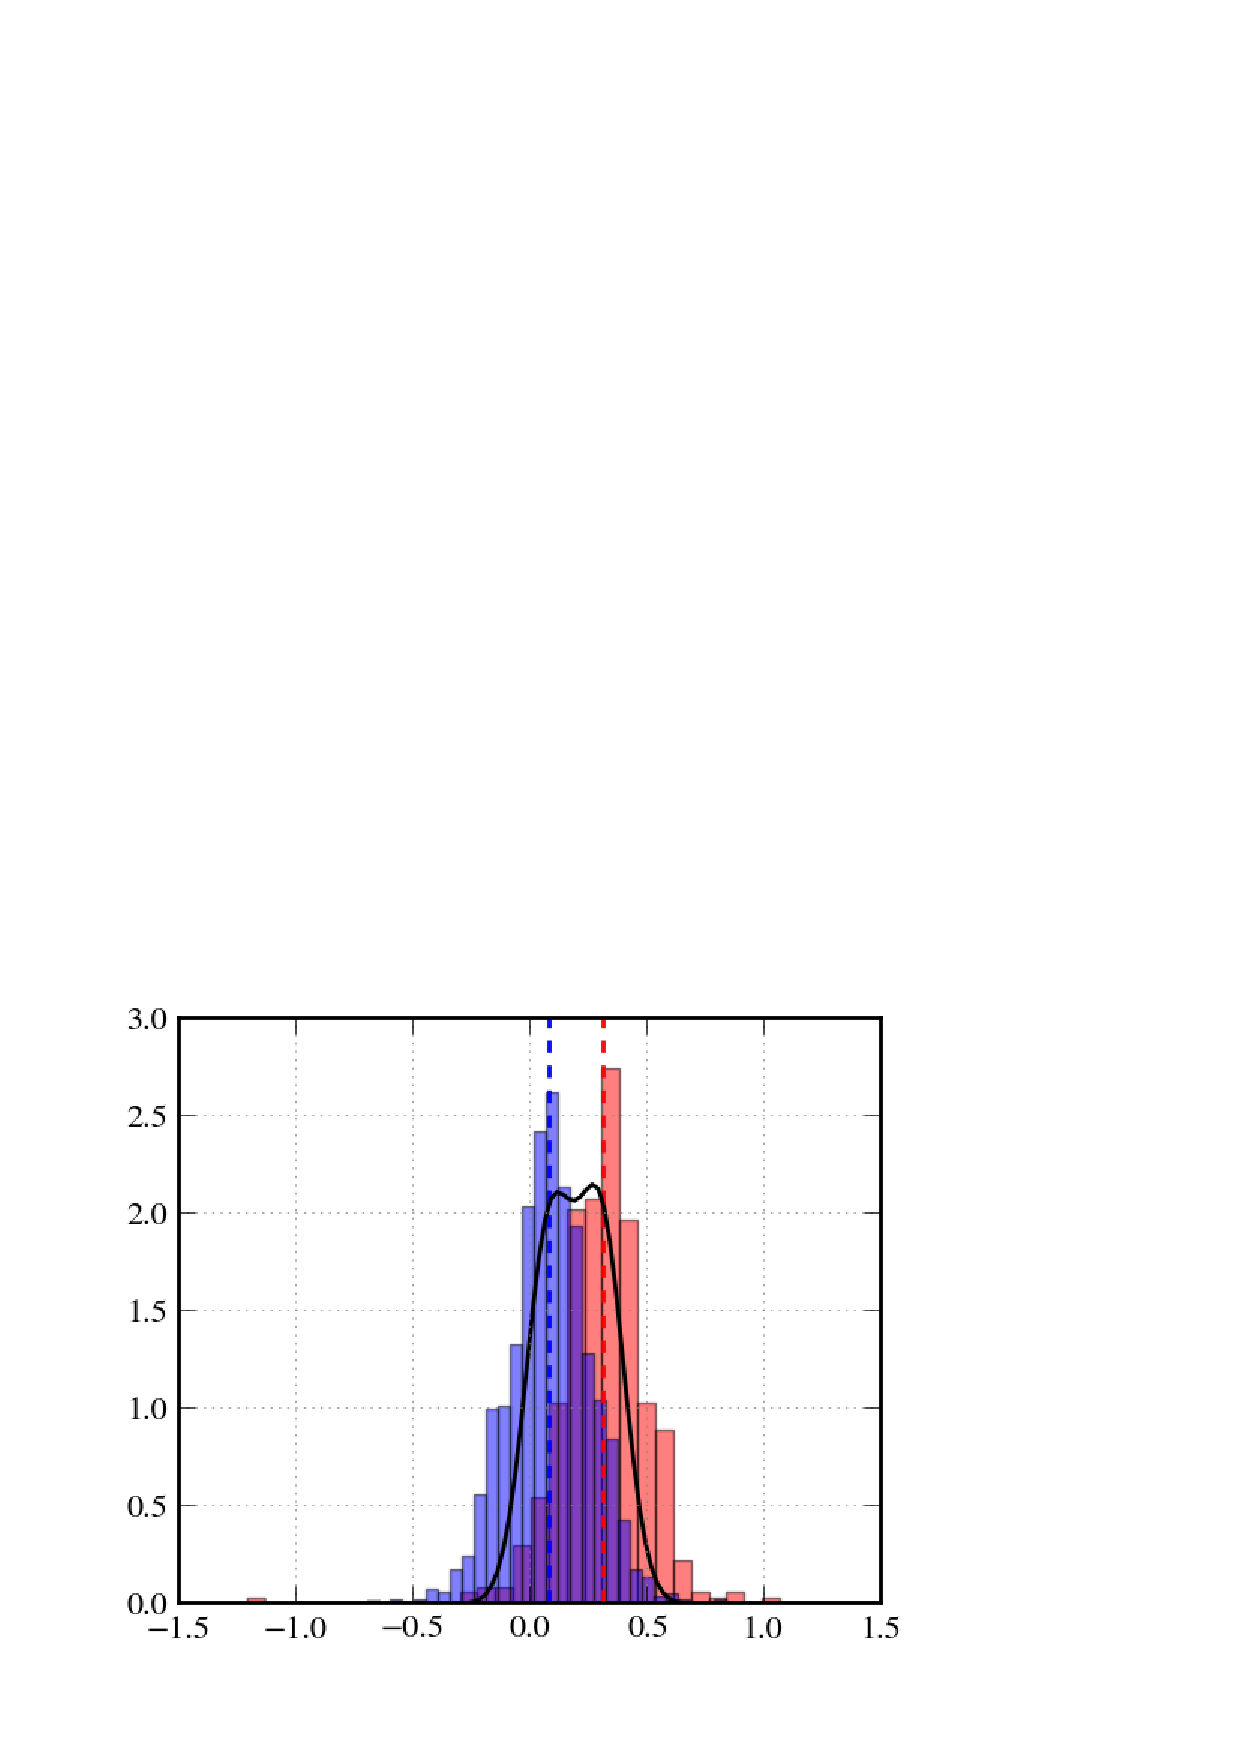
\includegraphics[width=0.5\textwidth]{fig/pymcmetals.png}
\caption{Distribution function of two populations (filled histograms) and the reproduced overall distribution.}
\label{fig:pops}
\end{center}
\end{figure*}

The routine then assigns each particle to one of the two populations,
based on its Mg metallicity. The procedure assigns $75\pm4\%$ of all
stars to the correct underlying distribution. This in turn changes the
half-light radius by $110$pc and $-62$pc for initial 390 pc, 730 pc
half light radii. These changes are rather high, but the two
populations still show distinct half-light radii.
